\documentclass[table]{beamer}

\usepackage{pucv_jz}

\title{Test de Hipótesis}
\subtitle{Estadística Computacional}
\author[J.Z.O-2023]{Juan Zamora Osorio\\\url{juan.zamora@pucv.cl}}
\institute[PUCV]{Instituto de Estadística\\Pontificia Universidad Cat\'olica de Valpara\'iso}
\date{\today}

\begin{document}

% Needed to reduce waste of blank space after block titles
\addtobeamertemplate{block begin}{\setlength\abovedisplayskip{0pt}}

\begin{frame}[plain]
    \titlepage
\end{frame}

\begin{frame}
    \frametitle{Test de Hipótesis}
    \begin{block}{Hemos aprendido sobre...}
        \begin{itemize}
            \item Describir datos.
            \item Probabilidades.
            \item Variables aleatorias.
            \item Inferencia estadística (paramétros).
        \end{itemize}
    \end{block}
    \begin{block}{Objetivo}
        \begin{itemize}
            \item Comparar \emph{hipótesis} o afirmaciones sobre una característica de una población.
            \item Características:
                \begin{itemize}
                    \item Valor de un parámetro de la población.
                    \item Valor de varios parámetros de la población.
                    \item Forma de la distribución de un parámetro de la población o de la población misma.
                \end{itemize}
        \end{itemize}
    \end{block}
\end{frame}

\begin{frame}
    \frametitle{Recordar}
    \begin{block}{Probabilidades}
        \begin{itemize}
            \item ¿Dado un proceso que genera datos, cuáles son las propiedades que observaremos?
        \end{itemize}
    \end{block}
    \begin{center}
        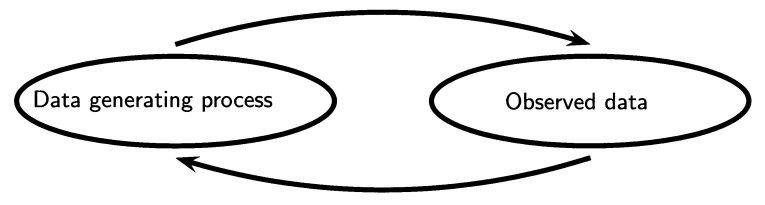
\includegraphics[height=0.3\textheight]{all2014_probabilidad_vs_inferencia}
    \end{center}
    \begin{block}{Inferencia estadística}
        \begin{itemize}
            \item ¿Dadas las observaciones, qué podemos decir sobre el proceso que genera los datos?
        \end{itemize}
    \end{block}
\end{frame}

\begin{frame}
    \frametitle{Ejemplo: Descubrimiento Bosson de Higgs}
    \begin{center}
        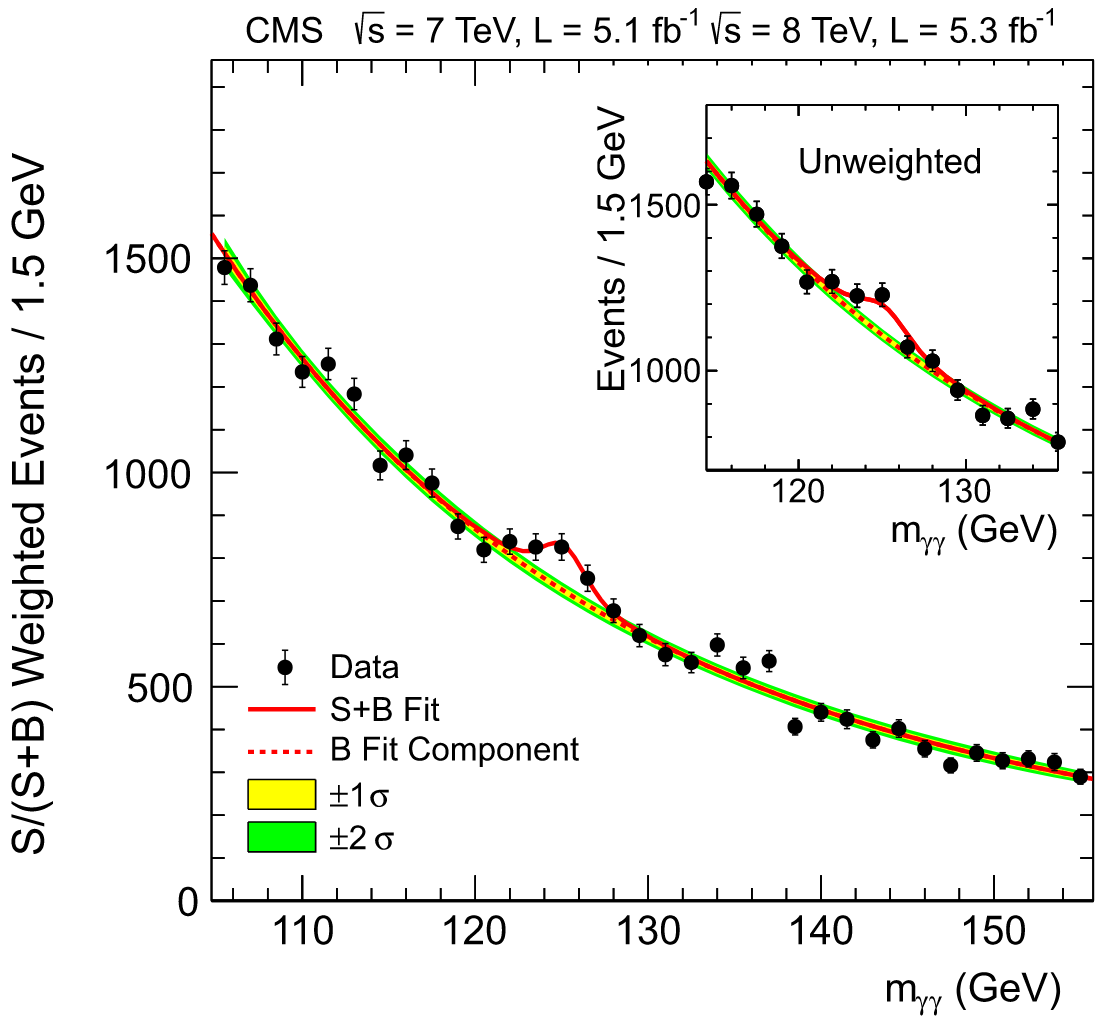
\includegraphics[height=0.87\textheight]{higgs_example1}
    \end{center}
\end{frame}

\begin{frame}
    \frametitle{Ejemplo: A/B testing}
    \begin{center}
        
\includegraphics[height=0.87\textheight]{abtesting_2}
    \end{center}
\end{frame}

\begin{frame}
    \frametitle{Ejemplo: A/B testing}
    \begin{center}
        
\includegraphics[width=\textwidth]{abtesting_1}
    \end{center}
\end{frame}

\begin{frame}
    \frametitle{Hipótesis}
    \begin{block}{Hipótesis nula $H_{0}$}
        \begin{itemize}
            \item Una afirmación supuesta como verdad hasta ahora.
            \item Supuesto a priori.
        \end{itemize}
    \end{block}
    \begin{block}{Hipótesis alternativa $H_{1}$ o $H_{\text{a}}$}
        \begin{itemize}
            \item Una afirmación distinta a $H_{0}$.
            \item Generalmente $H_{1}$ contradice $H_{0}$.
        \end{itemize}
    \end{block}
    \begin{block}{Test de hipótesis}
        \begin{itemize}
            \item Hipótesis $H_{0}$ debe ser \emph{falsable}.
            \item Se busca rechazar $H_{0}$ en favor de $H_{1}$.
            \item Respuestas: se rechaza, o no se puede rechazar.
        \end{itemize}
    \end{block}
\end{frame}

\begin{frame}
    \frametitle{Hipótesis}
    \begin{alertblock}{Cuidado}
        \begin{itemize}
            \item ¡Rechazar no es lo mismo que aceptar!
            \item Muchos tests se basan en rechazar o no una hipótesis, sin mirar la alternativa.
        \end{itemize}
    \end{alertblock}
    \begin{alertblock}{Cuidado}
        \begin{itemize}
            \item Generalmente es más útil saber qué hipótesis es más plausible (contraste de hipótesis).
            \item No veremos relaciones de causalidad en este curso.
        \end{itemize}
    \end{alertblock}
    \begin{block}{Incertidumbre}
        \begin{itemize}
            \item ¿Podemos cuantificar el grado de rechazo de una hipótesis?
            \item Si conseguimos más datos, ¿podemos responder?
        \end{itemize}
    \end{block}
\end{frame}

\begin{frame}
    \frametitle{Hipótesis -- región crítica}
    \begin{block}{Recordar: Estadístico}
        \begin{itemize}
            \item Sea $\Xvec$ una muestra iid univariada.
            \item Recordar que un estadístico es una función de la muestra.
            \item El estadístico tiene una distribución que depende de la muestra.
        \end{itemize}
    \end{block}
    \begin{block}{Regla de decisión}
        \begin{itemize}
            \item Si el estadístico cae en la \emph{región crítica}, se rechaza $H_{0}$.
        \end{itemize}
    \end{block}
    \begin{exampleblock}{Ejemplo}
        \begin{itemize}
            \item $H_{0} =$ la altura media de lo/as estudiantes del departamento de informática es mayor a $1.65$ m.
            \item Se mide la altura de $25$ estudiantes de este curso.
            \item Se calcula el promedio (media muestral $\bar{X}_{25}$).
            \item La región crítica es el rango de valores de $\bar{X}_{25}$ donde $H_{0}$ se rechaza.
        \end{itemize}
    \end{exampleblock}
\end{frame}

\begin{frame}
    \frametitle{Hipótesis -- errores}
    \begin{block}{Error de tipo I}
        \begin{itemize}
            \item Se rechaza la hipótesis nula cuando en verdad es cierta.
            \item Se suele llamar \emph{nivel de significancia}.
        \end{itemize}
    \end{block}
    \begin{block}{Error de tipo II}
        \begin{itemize}
            \item No se rechaza la hipótesis nula cuando en verdad es falsa.
        \end{itemize}
    \end{block}
\end{frame}

\begin{frame}
    \frametitle{Hipótesis -- errores}
    \begin{exampleblock}{Ejemplo}
        \begin{itemize}
            \item Supongamos que la altura sigue distribución normal $\normal{\mu}{0.01}$.
            \item Supongamos que rechazamos si $\bar{X}_{25} < 1.70$.
            \item Supongamos que $\mu$ tiene distribución a priori uniforme entre $0$ y $3$
        \end{itemize}
    \end{exampleblock}

\end{frame}

\begin{frame}
	\textit{(Continuación del ejemplo...)}
    \begin{block}{Probabilidad de error de tipo I}
        \begin{itemize}
            \item Por teorema del límite central, sabemos que $\bar{X}_{25} \sim \normal{\mu}{\frac{0.01}{25}}$.
        \end{itemize}
        \begin{multline*}
            \prob{\text{error de tipo I}}
            = \prob{\text{rechazar } H_{0} \mid H_{0} \text{ es cierta}}
            \\
            = \prob{\bar{X}_{n} < 1.70 \mid \mu > 1.65}
            = \frac{\prob{\bar{X}_{n} < 1.70 , \mu > 1.65}}{\prob{\mu > 1.65}}
            \\
            = \frac{\int_{1.65}^{3} \phifunc{5 \frac{1.7 - \mu}{0.1}} \pdf{\mu} d \mu}{\int_{1.65}^{3} \pdf{\mu} d \mu}
            = \frac{1}{3 - 1.65} \int_{1.65}^{3} \phifunc{50 \parens{1.7 - \mu}} d \mu \approx 0.037 .
        \end{multline*}
    \end{block}

\end{frame}

\begin{frame}
    \frametitle{Hipótesis -- errores}
    \begin{exampleblock}{Ejemplo}
        \begin{itemize}
            \item Supongamos que la altura sigue distribución normal $\normal{\mu}{0.01}$.
            \item Supongamos que rechazamos si $\bar{X}_{25} < 1.70$.
            \item Supongamos que $\mu$ tiene distribución a priori uniforme entre $0$ y $3$
        \end{itemize}
    \end{exampleblock}
    
\end{frame}

\begin{frame}
\textit{(Continuación del ejemplo...)}
    \begin{block}{Probabilidad de error de tipo II}
        \begin{itemize}
            \item Por teorema del límite central, sabemos que $\bar{X}_{25} \sim \normal{\mu}{\frac{0.01}{25}}$.
        \end{itemize}
        \begin{multline*}
            \prob{\text{error de tipo I}}
            = \prob{\text{no rechazar } H_{0} \mid H_{0} \text{ no es cierta}}
            \\
            = \prob{\bar{X}_{n} \geq 1.70 \mid \mu \leq 1.65}
            %= \frac{\prob{\bar{X}_{n} < 1.70 , \mu \leq 1.65}}{\prob{\mu \leq 1.65}}
            = \frac{\int_{0}^{1.65} \parens{1 - \phifunc{5 \frac{1.7 - \mu}{0.1}}} \pdf{\mu} d \mu}{\int_{0}^{1.65} \pdf{\mu} d \mu}
            \\
            = \frac{1}{1.65 - 0} \int_{0}^{1.65} 1 - \phifunc{50 \parens{1.7 - \mu}} d \mu \approx 0.000024 .
        \end{multline*}
    \end{block}
\end{frame}

\begin{frame}
    \frametitle{Hipótesis -- errores}
    \begin{block}{Errores}
        \begin{itemize}
            \item Tipo I: se rechaza la hipótesis nula cuando en verdad es cierta.
            \item Tipo II: no se rechaza la hipótesis nula cuando en verdad es falsa.
        \end{itemize}
    \end{block}

\end{frame}

\begin{frame}
    \begin{exampleblock}{Ejemplo}
        \begin{itemize}
            \item $H_{0} =$ la altura media de lo/as estudiantes del departamento de informática es mayor a $1.65$ m.
                \begin{itemize}
                    \item $\prob{\text{error de tipo I}} = \prob{\text{rechazar } H_{0} \mid H_{0} \text{ es cierta}} \approx 0.037$.
                    \item $\prob{\text{error de tipo II}}
                        = \prob{\text{no rechazar } H_{0} \mid H_{0} \text{ no es cierta}} \approx 0.000024$.
                \end{itemize}
            \item Ambas dependen del umbral de corte $t$. En el ejemplo, $t = 1.7$.
            \item Podemos variar $t$ de manera de reducir alguno de los dos.
                \begin{itemize}
                    \item Si $t$ aumenta, el error de tipo I aumenta y el error de tipo II disminuye.
                    \item Si $t$ disminuye, el error de tipo I disminuye y el error de tipo II aumenta.
                \end{itemize}
        \end{itemize}
    \end{exampleblock}
\end{frame}

\begin{frame}
    \frametitle{Ejemplo: recuperación de enfermedad}
    \begin{exampleblock}{Probando un medicamento}
        \begin{itemize}
            \item Se sabe que si una persona contrae una enfermedad, tiene probabilidad $p = 0.25$ de sobrevivir luego de $3$ meses.
            \item Se experimenta un nuevo remedio en $20$ personas recién contagiadas.
            \item Luego de $3$ meses se revisa cuántos sobrevivieron.
            \item La hipótesis nula $H_{0}$ es que el remedio no afecta, por lo que la nueva probabilidad de sobrevivir luego de $3$ meses es $p = 0.25$.
            \item La hipótesis alternativa $H_{1}$ es que la probabilidad es mayor, $p > 0.25$.
            \item ¿Cuántas personas deberían sobrevivir para rechazar $H_{0}$?
        \end{itemize}
    \end{exampleblock}
\end{frame}

\begin{frame}
    \frametitle{Ejemplo: recuperación de enfermedad}
    \begin{exampleblock}{Probando un medicamento}
        \begin{itemize}
            \item Se sabe que si una persona contrae una enfermedad, tiene probabilidad $p = 0.25$ de sobrevivir luego de $3$ meses.
            \item Se experimenta un nuevo remedio en $20$ personas recién contagiadas.
            \item La hipótesis nula $H_{0}$ es que el remedio no afecta, por lo que la nueva probabilidad de sobrevivir luego de $3$ meses es $p = 0.25$.
            \item La hipótesis alternativa $H_{1}$ es que la probabilidad es mayor, $p > 0.25$.
            \item ¿Cuántas personas deberían sobrevivir para rechazar $H_{0}$?
        \end{itemize}
    \end{exampleblock}

\end{frame}

\begin{frame}
    \begin{block}{Desarrollo}
        \begin{itemize}
            \item Estadístico: $X$ cantidad de personas que sobrevivieron.
            \item $X$ sigue una distribución binomial $\binomial{n}{p}$.
                \begin{multline*}
                    \prob{\text{error de tipo I}} = \prob{\text{rechazar } H_{0} \mid H_{0} \text{ es cierta}}
                    \\
                    = \prob{X \geq t \mid p = 0.25} = 1 - \pFF{X \sim \binomial{20}{0.25}}{t - 1} .
                \end{multline*}
        \end{itemize}
    \end{block}
\end{frame}

\begin{frame}
    \frametitle{Ejemplo: recuperación de enfermedad}
    \begin{exampleblock}{Probando un medicamento}
        \begin{itemize}
            \item Se sabe que si una persona contrae una enfermedad, tiene probabilidad $p = 0.25$ de sobrevivir luego de $3$ meses.
            \item Se experimenta un nuevo remedio en $20$ personas recién contagiadas.
            \item La hipótesis nula $H_{0}$ es que el remedio no afecta, por lo que la nueva probabilidad de sobrevivir luego de $3$ meses es $p = 0.25$.
            \item La hipótesis alternativa $H_{1}$ es que la probabilidad es mayor, $p > 0.25$.
            \item ¿Cuántas personas deberían sobrevivir para rechazar $H_{0}$?
        \end{itemize}
    \end{exampleblock}

\end{frame}

\begin{frame}
    \begin{block}{Desarrollo}
        \begin{itemize}
            \item Estadístico: $X$ cantidad de personas que sobrevivieron.
            \item $X$ sigue una distribución binomial $\binomial{n}{p}$.
                \begin{multline*}
                    \prob{\text{error de tipo II}} = \prob{\text{no rechazar } H_{0} \mid H_{0} \text{ no es cierta}}
                    \\
                    = \prob{X < t \mid p \neq 0.25}
                    = \pFF{X \sim \binomial{20}{p}}{t - 1} .
                \end{multline*}
        \end{itemize}
    \end{block}
\end{frame}

\begin{frame}
    \frametitle{Ejemplo: recuperación de enfermedad}
    \begin{block}{¿Cuál punto de corte $t$ para rechazar?}
        \begin{itemize}
            \item $\prob{\text{error de tipo I}} = \prob{\text{rechazar } H_{0} \mid H_{0} \text{ es cierta}}
                    = 1 - \pFF{X \sim \binomial{20}{0.25}}{t - 1}$.
            \item $\prob{\text{error de tipo II}} = \prob{\text{no rechazar } H_{0} \mid H_{0} \text{ no es cierta}} = \pFF{X \sim \binomial{20}{p}}{t - 1}$.
        \end{itemize}
    \end{block}
    \begin{exampleblock}{Ejemplo: $t = 9$}
        \begin{itemize}
            \item $\prob{\text{error de tipo I}} = \prob{\text{rechazar } H_{0} \mid H_{0} \text{ es cierta}}
                    \approx 0.0409$.
            \item $\prob{\text{error de tipo II}} = \prob{\text{no rechazar } H_{0} \mid H_{0} \text{ no es cierta}} =$
                \begin{center}
                    \begin{tabular}{c|cccc}
                        $p$ & $0.25$ & $0.3$ & $0.5$ & $0.75$ \\
                        \hline
                        $\prob{\text{error de tipo II}}$ & $0.9591$ & $0.8867$ & $0.2517$ & $0.0009$
                    \end{tabular}
                \end{center}
        \end{itemize}
    \end{exampleblock}
    \begin{center}
        \begin{tikzpicture}
            \begin{axis}[
                axis x line=bottom,
                axis y line=none,
                xtick distance=1,
                height=2.5cm, width=\textwidth
                ]
                \addplot [blue, name path=A] coordinates {(0, 0) (0, 4) (20, 4) (20, 0)};
                \addplot [name path=B] coordinates {(0, 0) (20, 0)};
                \addplot [blue!30] fill between [of=A and B, soft clip={domain=0:8.5}];
                \addplot [orange!30] fill between [of=A and B, soft clip={domain=8.5:20}];
                \node at (axis cs:4, 2) {No rechazar $H_{0}$};
                \node at (axis cs:14, 2) {Rechazar $H_{0}$};
            \end{axis}
        \end{tikzpicture}
    \end{center}
\end{frame}

\begin{frame}
    \frametitle{Ejemplo: recuperación de enfermedad}
    \begin{block}{¿Cuál punto de corte $t$ para rechazar?}
        \begin{itemize}
            \item $\prob{\text{error de tipo I}} = \prob{\text{rechazar } H_{0} \mid H_{0} \text{ es cierta}}
                    = 1 - \pFF{X \sim \binomial{20}{0.25}}{t - 1}$.
            \item $\prob{\text{error de tipo II}} = \prob{\text{no rechazar } H_{0} \mid H_{0} \text{ no es cierta}} = \pFF{X \sim \binomial{20}{p}}{t - 1}$.
        \end{itemize}
    \end{block}
    \begin{exampleblock}{Ejemplo: $t = 8$}
        \begin{itemize}
            \item $\prob{\text{error de tipo I}} = \prob{\text{rechazar } H_{0} \mid H_{0} \text{ es cierta}}
                    \approx 0.1018$.
            \item $\prob{\text{error de tipo II}} = \prob{\text{no rechazar } H_{0} \mid H_{0} \text{ no es cierta}} =$
                \begin{center}
                    \begin{tabular}{c|cccc}
                        $p$ & $0.25$ & $0.3$ & $0.5$ & $0.75$ \\
                        \hline
                        $\prob{\text{error de tipo II}}$ & $0.8982$ & $0.7723$ & $0.1316$ & $0.0002$
                    \end{tabular}
                \end{center}
        \end{itemize}
    \end{exampleblock}
    \begin{center}
        \begin{tikzpicture}
            \begin{axis}[
                axis x line=bottom,
                axis y line=none,
                xtick distance=1,
                height=2.5cm, width=\textwidth
                ]
                \addplot [blue, name path=A] coordinates {(0, 0) (0, 4) (20, 4) (20, 0)};
                \addplot [name path=B] coordinates {(0, 0) (20, 0)};
                \addplot [blue!30] fill between [of=A and B, soft clip={domain=0:7.5}];
                \addplot [orange!30] fill between [of=A and B, soft clip={domain=7.5:20}];
                \node at (axis cs:4, 2) {No rechazar $H_{0}$};
                \node at (axis cs:14, 2) {Rechazar $H_{0}$};
            \end{axis}
        \end{tikzpicture}
    \end{center}
\end{frame}

\begin{frame}
    \frametitle{Ejemplo: peso de recién nacido/as}
    \begin{exampleblock}{Comparando países}
        \begin{itemize}
            \item Se sabe que recién nacidos en Inglaterra tienen peso con media $3$ kg y desviación estándar de $0.5$ kg.
            \item Se cree que la media de peso de recién nacidos en Australia es mayor.
            \item $H_{0}$: la media de peso en Australia es similar a la de Inglaterra, $3$ kg.
            \item $H_{1}$: la media de peso en Australia es significativamente mayor a $3$ kg.
        \end{itemize}
    \end{exampleblock}
    \begin{block}{Desarrollo}
        \begin{itemize}
            \item $H_{0}: \mu = 3$ kg.
            \item $H_{1}: \mu > 3$ kg.
            \item Se obtiene una muestra de $44$ recién nacidos (conjunto \emph{Babyboom}).
        \end{itemize}
    \end{block}
\end{frame}

\begin{frame}
    \frametitle{Ejemplo: peso de recién nacido/as}
    \begin{block}{44 recién nacidos: conjunto \emph{Babyboom}}
        \begin{itemize}
            \item Media muestral $\bar{x}_{44} \approx 3.276$.
            \item Si $H_{0}$ es cierta, $\prob{\text{error de tipo I}} = \prob{\bar{X}_{44} > 3.276 \mid \mu = 3}$
        \end{itemize}
    \end{block}
    \begin{center}
        \begin{tikzpicture}
            \begin{axis}[
                height=0.5\textwidth,
                width=0.81\textwidth,
                    ybar interval,
                    xtick=,
                    xticklabel={$\left [ \pgfmathprintnumber\tick, \pgfmathprintnumber\nexttick \right )$},
                    ylabel={Frecuencia absoluta},
                    xlabel={Peso (kg)},
                axis x line=bottom,
                axis y line=left
            ]
                \addplot+ [hist={data=x / 1000}] file {babyboom/weight.dat};
            \end{axis}
        \end{tikzpicture}
    \end{center}
\end{frame}

\begin{frame}
    \frametitle{Ejemplo: peso de recién nacido/as}
    \begin{block}{44 recién nacidos: conjunto \emph{Babyboom}}
        \begin{itemize}
            \item Media muestral $\bar{x}_{44} \approx 3.276$.
            \item Si $H_{0}$ es cierta, $\prob{\text{error de tipo I}} = \prob{\bar{X}_{44} > 3.276 \mid \mu = 3}$
            \item Por teorema del límite central, $\bar{X}_{44} \sim \normal{\mu}{\frac{\sigma^{2}}{n}} = \normal{3}{\frac{0.25}{44}}$.
            \item Entonces, $\prob{\bar{X}_{44} > 3.276 \mid \mu = 3} = 1 - \pFF{\bar{X}_{44} \sim \normal{3}{\frac{1}{176}}}{3.276}$.
            \item Es decir, $\prob{\bar{X}_{44} > 3.276 \mid \mu = 3} \approx 0.000125$.
        \end{itemize}
    \end{block}
    \begin{center}
        \begin{tikzpicture}[
                declare function={normal(\x,\m,\s) = 1 / (\s * sqrt(2 * pi)) * exp(-(\x-\m)^2 / (2 * \s^2));}]
            \begin{axis}[
                height=0.31\textwidth,
                width=0.5\textwidth,
                    xlabel={Peso (kg)},
                axis x line=bottom,
                axis y line=none,
                ymin=0,
                samples=50
            ]
                \addplot [blue, domain=2.6:3.4, name path=A] {normal(x, 3, sqrt(1 / 176))};
                \addplot [name path=B] coordinates {(3, 0) (3.4, 0)};
                \addplot [blue!30] fill between [of=A and B, soft clip={domain=3.276:3.4}];
                \draw (axis cs:3, 0) -- (axis cs:3, 5.292567428401227);
            \end{axis}
        \end{tikzpicture}
        \begin{tikzpicture}[
                declare function={normal(\x,\m,\s) = 1 / (\s * sqrt(2 * pi)) * exp(-(\x-\m)^2 / (2 * \s^2));}]
            \begin{axis}[
                height=0.31\textwidth,
                width=0.5\textwidth,
                    xlabel={Peso (kg)},
                axis x line=bottom,
                axis y line=none,
                ymin=0,
                samples=50
            ]
                \addplot [blue, domain=3.25:3.35, name path=A] {normal(x, 3, sqrt(1 / 176))};
                \addplot [name path=B] coordinates {(3.25, 0) (3.35, 0)};
                \addplot [blue!30] fill between [of=A and B, soft clip={domain=3.276:3.35}];
                \node [pin=90:{}] at (axis cs:3.285, 0.001) {};
                \node at (axis cs:3.307, 0.012) {$\prob{\bar{X}_{44} > 3.276 \mid \mu = 3}$};
            \end{axis}
        \end{tikzpicture}
    \end{center}
\end{frame}

\begin{frame}
    \frametitle{Ejemplo: peso de recién nacido/as}
    \begin{block}{p-valor}
        \begin{itemize}
            \item Media muestral $\bar{x}_{44} \approx 3.276$.
            \item $\prob{\bar{X}_{44} > 3.276 \mid \mu = 3} \approx 0.000125$ es llamado \emph{p-valor}.
            \item El p-valor indica la probabilidad de encontrar un resultado como el obtenido si $H_{0}$ es cierta.
        \end{itemize}
    \end{block}
    \begin{center}
        \begin{tikzpicture}[
                declare function={normal(\x,\m,\s) = 1 / (\s * sqrt(2 * pi)) * exp(-(\x-\m)^2 / (2 * \s^2));}]
            \begin{axis}[
                height=0.31\textwidth,
                width=0.5\textwidth,
                    xlabel={Peso (kg)},
                axis x line=bottom,
                axis y line=none,
                ymin=0,
                samples=50
            ]
                \addplot [blue, domain=2.6:3.4, name path=A] {normal(x, 3, sqrt(1 / 176))};
                \addplot [name path=B] coordinates {(3, 0) (3.4, 0)};
                \addplot [blue!30] fill between [of=A and B, soft clip={domain=3.276:3.4}];
                \draw (axis cs:3, 0) -- (axis cs:3, 5.292567428401227);
            \end{axis}
        \end{tikzpicture}
        \begin{tikzpicture}[
                declare function={normal(\x,\m,\s) = 1 / (\s * sqrt(2 * pi)) * exp(-(\x-\m)^2 / (2 * \s^2));}]
            \begin{axis}[
                height=0.31\textwidth,
                width=0.5\textwidth,
                    xlabel={Peso (kg)},
                axis x line=bottom,
                axis y line=none,
                ymin=0,
                samples=50
            ]
                \addplot [blue, domain=3.25:3.35, name path=A] {normal(x, 3, sqrt(1 / 176))};
                \addplot [name path=B] coordinates {(3.25, 0) (3.35, 0)};
                \addplot [blue!30] fill between [of=A and B, soft clip={domain=3.276:3.35}];
                \node [pin=90:{}] at (axis cs:3.285, 0.001) {};
                \node at (axis cs:3.307, 0.012) {$\prob{\bar{X}_{44} > 3.276 \mid \mu = 3}$};
            \end{axis}
        \end{tikzpicture}
    \end{center}
    \begin{block}{Nivel de significancia}
        \begin{itemize}
            \item Generalmente se elige de antemano un $\alpha$ máximo.
        \end{itemize}
    \end{block}
\end{frame}

\begin{frame}
    \begin{center}
        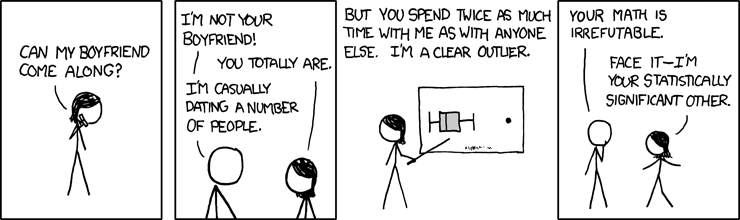
\includegraphics[width=\textwidth]{boyfriend}
    \end{center}
\end{frame}

\begin{frame}
    \frametitle{Varianza desconocida}
    \begin{exampleblock}{Comparando países}
        \begin{itemize}
            \item Se sabe que recién nacidos en Inglaterra tienen peso con media $3$ kg.
            \item Se cree que la media de peso de recién nacidos en Australia es mayor.
            \item $H_{0}$: la media de peso en Australia similar a Inglaterra, $3$ kg.
            \item $H_{1}$: la media de peso en Australia significativamente $>3$ kg.
        \end{itemize}
    \end{exampleblock}
    \begin{block}{Desarrollo}
        \begin{itemize}
            \item $H_{0}: \mu = 3$ kg.
            \item $H_{1}: \mu > 3$ kg.
            \item Se obtiene una muestra de $44$ recién nacidos (conjunto \emph{Babyboom}).
            \item $\bar{x}_{44} \approx 3.276$.
            \item $\sqrt{s^{2}_{44}} \approx 0.5280$.
        \end{itemize}
    \end{block}
\end{frame}

\begin{frame}
    \frametitle{Varianza desconocida}
    \begin{block}{Recuerdo}
        \begin{itemize}
            \item La variable aleatoria $T = \frac{\sqrt{n} \parens{\bar{X}_{n} - \mu}}{\sqrt{S^{2}_{n}}}$ tiene distribución $t$ de Student con $n - 1$ grados de libertad.
        \end{itemize}
    \end{block}
    \begin{block}{Desarrollo}
        \begin{itemize}
            \item $\bar{x}_{44} \approx 3.276$.
            \item $\sqrt{s^{2}_{44}} \approx 0.5280$.
            \item $t = \frac{\sqrt{44} \parens{3.276 - \mu}}{0.5280} \approx 3.4674$
            \item $\prob{\text{error de tipo I}} = \prob{T > t \mid \mu = 3} \approx \prob{T > 3.4674}$.
            \item Es decir, $\prob{\text{error de tipo I}} = 1 - \prob{T \leq 3.4674} \approx 0.0006$.
            \item Si se considera $\alpha = 0.01$, se rechaza $H_{0}$.
        \end{itemize}
    \end{block}
\end{frame}

\begin{frame}
    \frametitle{Ejemplo: peso de recién nacido/as}
    \begin{block}{p-valor}
        \begin{itemize}
            \item En el caso de varianza conocida, p-valor es $0.00013$.
            \item En el caso de varianza desconocia, p-valor es $0.0006$.
            \item Distribución $t$ de Student tiene colas anchas, en comparación con normal.
        \end{itemize}
    \end{block}
    \begin{block}{Definir región crítica}
        \begin{itemize}
            \item Se podría elegir nivel de significancia $\alpha$ de antemano.
            \item Luego calcular para qué valor de $\bar{X}_{n}$ se rechaza la hipótesis.
        \end{itemize}
    \end{block}
    \begin{center}
        \begin{tikzpicture}[
                declare function={normal(\x,\m,\s) = 1 / (\s * sqrt(2 * pi)) * exp(-(\x-\m)^2 / (2 * \s^2));}]
            \begin{axis}[
                height=0.31\textwidth,
                width=0.5\textwidth,
                axis x line=bottom,
                axis y line=none,
                xtick={0, 1},
                xticklabels={$\mu$, $c$},
                ymin=0,
                samples=50
            ]
                \addplot [blue, domain=-1:3, name path=A] {normal(x, 0, 1)};
                \addplot [name path=B] coordinates {(-1, 0) (3, 0)};
                \addplot [blue!30] fill between [of=A and B, soft clip={domain=1:3}];
                %\node [pin=90:{}] at (axis cs:2, 0.001) {};
                %\node at (axis cs:2.2, 0.21) {$\prob{\bar{X}_{n} > c} = \alpha$};
                \node [pin=90:{$\prob{\bar{X}_{n} > c} = \alpha$}] at (axis cs:1.8, 0.15) {};
            \end{axis}
        \end{tikzpicture}
    \end{center}
\end{frame}

\begin{frame}
    \begin{center}
        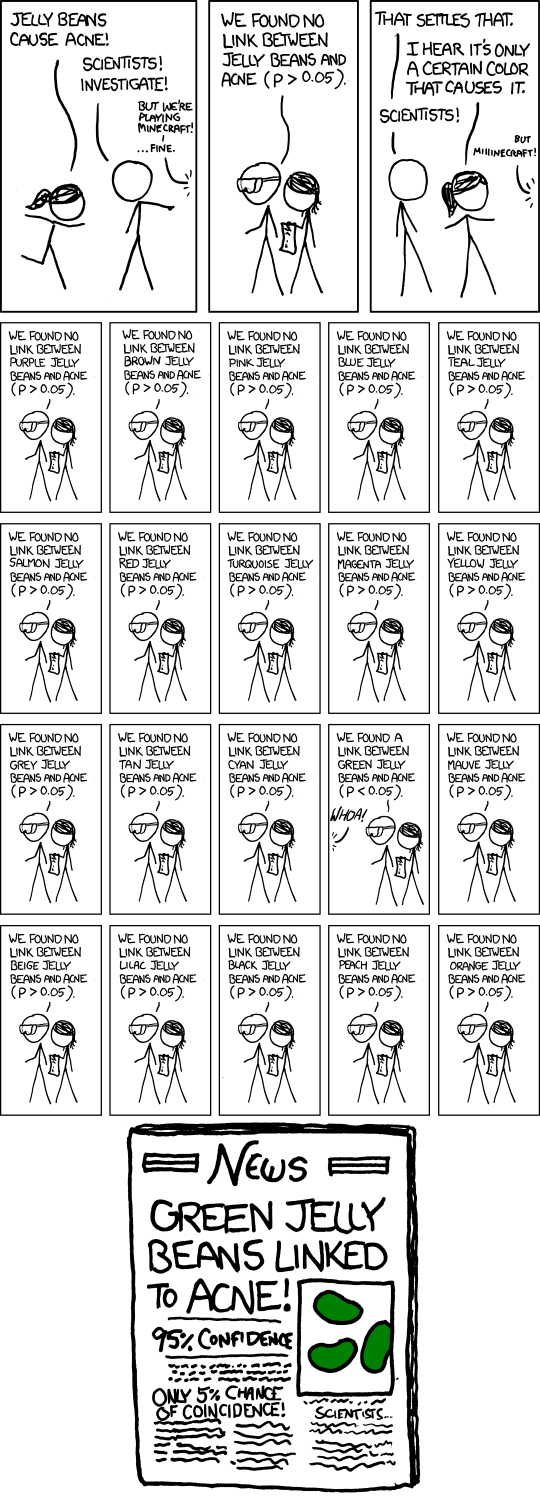
\includegraphics[height=0.96\textheight]{significant}
    \end{center}
\end{frame}

\begin{frame}
    \frametitle{Bilateral (\emph{two sided})}
    \begin{exampleblock}{Comparando países}
        \begin{itemize}
            \item Se sabe que recién nacidos en Inglaterra tienen peso con media $3$ kg.
            \item Se cree que media de peso de recién nacidos en Australia es distinta.
            \item $H_{0}$: la media de peso en Australia es similar a la de Inglaterra, $3$ kg.
            \item $H_{1}$: la media de peso en Australia es significativamente distinta a $3$ kg.
        \end{itemize}
    \end{exampleblock}

\end{frame}

\begin{frame}
    \begin{block}{Desarrollo}
        \begin{itemize}
            \item $H_{0}: \mu = 3$ kg.
            \item $H_{1}: \mu \neq 3$ kg.
            \item Se obtiene una muestra de $44$ recién nacidos (conjunto \emph{Babyboom}).
            \item $\bar{x}_{44} \approx 3.276$.
            \item $\sqrt{s^{2}_{44}} \approx 0.5280$.
        \end{itemize}
    \end{block}
\end{frame}

\begin{frame}
    \frametitle{Bilateral (\emph{two sided})}
    \begin{block}{Desarrollo}
        \begin{itemize}
            \item $H_{0}: \mu = 3$ kg.
            \item $H_{1}: \mu \neq 3$ kg.
            \item $\bar{x}_{44} \approx 3.276$, $\sqrt{s^{2}_{44}} \approx 0.5280$.
            \item Caso varianza desconocida: $t = \frac{\sqrt{44} \parens{3.276 - \mu}}{0.5280} \approx 3.4674$.
            \item $\prob{\vparens{T} > t} = \prob{T \leq - t} + \prob{T > t} = 1 + \prob{T \leq -t} - \prob{T \leq t}$.
            \item Así, $\prob{\vparens{T} > t} = 2 \prob{T \leq - \vparens{t}} \approx 0.0012$.
        \end{itemize}
    \end{block}
    \begin{center}
        \begin{tikzpicture}[
                declare function={normal(\x,\m,\s) = 1 / (\s * sqrt(2 * pi)) * exp(-(\x-\m)^2 / (2 * \s^2));}]
            \begin{axis}[
                height=0.31\textwidth,
                width=0.5\textwidth,
                axis x line=bottom,
                axis y line=none,
                xtick={-1.5, 0, 1.5},
                xticklabels={$\mu - c$, $\mu$, $\mu + c$},
                ymin=0,
                samples=50
            ]
                \addplot [blue, domain=-3:3, name path=A] {normal(x, 0, 1)};
                \addplot [name path=B] coordinates {(-3, 0) (3, 0)};
                \addplot [blue!30] fill between [of=A and B, soft clip={domain=1.5:3}];
                \addplot [blue!30] fill between [of=A and B, soft clip={domain=-3:-1.5}];
                %\node [pin=90:{}] at (axis cs:2, 0.001) {};
                %\node at (axis cs:2.2, 0.21) {$\prob{\bar{X}_{n} > c} = \alpha$};
                \node at (axis cs:0, 0.2) {$\prob{\vparens{\bar{X}_{n} - \mu} > c} = \alpha$};
            \end{axis}
        \end{tikzpicture}
    \end{center}
\end{frame}

\begin{frame}
    \frametitle{Ejemplo: peso de recién nacido/as}
    \begin{exampleblock}{44 recién nacidos: conjunto \emph{Babyboom}}
        \begin{itemize}
            \item El peso se puede diferenciar por género (masculino $M$ o femenino $F$).
            \item $18$ son femenino $F$, $26$ masculino $M$.
            \item Pesos promedio $\bar{x}^{F}_{18} \approx 3.132$, $\bar{x}^{M}_{26} \approx 3.375$.
            \item ¿Son las medias distintas significativamente?
        \end{itemize}
    \end{exampleblock}
    \begin{center}
        \begin{tikzpicture}
            \begin{axis}[
                height=0.4\textwidth,
                width=0.65\textwidth,
                ybar,
                    %ybar interval,
                    %xtick=,
                    %xticklabel={$\left [ \pgfmathprintnumber\tick, \pgfmathprintnumber\nexttick \right )$},
                   ylabel={Frecuencia absoluta},
                   xlabel={Peso (kg)},
                   legend entries={$F$,$M$},
                   legend pos={north west},
                axis x line=bottom,
                axis y line=left
            ]
                \addplot+ [opacity=0.5, hist={data=x / 1000, data max=4, data min=2}] file {babyboom/weightgirl.dat};
                \addplot+ [opacity=0.5, hist={data=x / 1000, data max=4, data min=2}] file {babyboom/weightboy.dat};
            \end{axis}
        \end{tikzpicture}
    \end{center}
\end{frame}

\begin{frame}
    \frametitle{Comparación de poblaciones}
    \begin{exampleblock}{44 recién nacidos: conjunto \emph{Babyboom}}
        \begin{itemize}
            \item El peso se puede diferenciar por género (masculino $M$ o femenino $F$).
            \item $18$ son femenino $F$, $26$ masculino $M$.
            \item Pesos promedio $\bar{x}^{F}_{18} \approx 3.132$, $\bar{x}^{M}_{26} \approx 3.375$.
            \item ¿Son las medias distintas significativamente?
        \end{itemize}
    \end{exampleblock}
    \begin{center}
        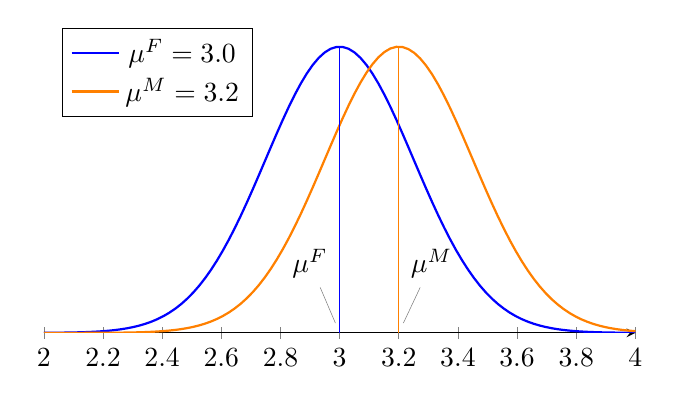
\begin{tikzpicture}[
                declare function={normal(\x,\m,\s) = 1 / (\s * sqrt(2 * pi)) * exp(-(\x - \m)^2 / (2 * \s^2));}]
            \begin{axis}[
                height=0.46\textwidth,
                width=0.75\textwidth,
                axis x line=bottom,
                axis y line=none,
                %xtick={0, 1},
                %xticklabels={$\mu$, $c$},
                ymin=0,
                legend entries={$\mu^{F} = 3.0$,$\mu^{M} = 3.2$},
                legend pos={north west},
                samples=100
            ]
                \addplot [blue, thick, domain=2:4] {normal(x, 3, 0.25)};
                \addplot [orange, thick, domain=2:4] {normal(x, 3.2, 0.25)};
                \draw[blue] (axis cs:3, 0) -- (axis cs:3, {normal(3, 3, 0.25)});
                \draw[orange] (axis cs:3.2, 0) -- (axis cs:3.2, {normal(3.2, 3.2, 0.25)});
                \node [pin=93:$\mu^{F}$] at (axis cs:3, 0) {};
                \node [pin=87:$\mu^{M}$] at (axis cs:3.2, 0) {};
            \end{axis}
        \end{tikzpicture}
    \end{center}
\end{frame}

\begin{frame}
    \frametitle{Comparación de poblaciones}
    \begin{block}{Desarrollo}
        \begin{itemize}
            \item $H_{0}: \mu^{M} = \mu^{F}$.
            \item $H_{1}: \mu^{M} \neq \mu^{F}$.
            \item Pesos promedio $\bar{x}^{F}_{18} \approx 3.132$, $\bar{x}^{M}_{26} \approx 3.375$.
        \end{itemize}
    \end{block}
    \begin{block}{Idea}
        \begin{itemize}
            \item Podemos contrastar la diferencia $\mu^{M} - \mu^{F}$ y $\bar{X}^{M}_{n} - \bar{X}^{F}_{m}$.
            \item $H_{0}: \mu^{M} - \mu^{F} = 0$.
            \item $H_{1}: \mu^{M} - \mu^{F} \neq 0$.
            \item Diferencia de promedios $\bar{x}^{M}_{26} - \bar{x}^{F}_{18} \approx 0.2429$.
            \item Si $H_{0}$ es cierta, ¿cómo se distribuye $\bar{X}^{M}_{n} - \bar{X}^{F}_{m}$?
        \end{itemize}
    \end{block}
\end{frame}

\begin{frame}
    \frametitle{Comparación de poblaciones}
    \begin{block}{Idea}
        \begin{itemize}
            \item $H_{0}: \mu^{M} - \mu^{F} = 0$.
            \item $H_{1}: \mu^{M} - \mu^{F} \neq 0$.
            \item Diferencia de promedios $\bar{x}^{M}_{26} - \bar{x}^{F}_{18} \approx 0.2429$.
            \item Si $H_{0}$ es cierta, ¿cómo se distribuye $\bar{X}^{M}_{n} - \bar{X}^{F}_{m}$?
        \end{itemize}
    \end{block}
    \begin{block}{Caso varianzas conocidas}
        \begin{itemize}
            \item $\bar{X}^{M}_{n} - \bar{X}^{F}_{m} \sim \normal{\mu^{M} - \mu^{F}}{\frac{\sigma^{2 M}}{n} + \frac{\sigma^{2 F}}{m}}$
            \item Se calcula $z = \frac{\bar{X}^{M}_{n} - \bar{X}^{F}_{m} - \mu^{M} + \mu^{F}}{\sqrt{\frac{\sigma^{2 M}}{n} + \frac{\sigma^{2 F}}{m}}}$.
            \item Se revisa p-valor $\prob{\vparens{Z} > z}$.
        \end{itemize}
    \end{block}
\end{frame}

\begin{frame}
    \frametitle{Comparación de poblaciones}
    \begin{block}{En el ejemplo}
        \begin{itemize}
            \item Diferencia de promedios $\bar{x}^{M}_{26} - \bar{x}^{F}_{18} \approx 0.2429$.
            \item Supongamos $\sigma^{2 M} = 0.5$ y $\sigma^{2 F} = 0.5$.
            \item $z = \frac{\bar{X}^{M}_{n} - \bar{X}^{F}_{m} - \mu^{M} + \mu^{F}}{\sqrt{\frac{\sigma^{2 M}}{n} + \frac{\sigma^{2 F}}{m}}} \approx 1.1201$.
            \item p-valor $\prob{\vparens{Z} > z} \approx 0.2627$.
        \end{itemize}
    \end{block}
\end{frame}

\begin{frame}
    \frametitle{Comparación de poblaciones}
    \begin{block}{Caso varianzas desconocidas: \emph{Welch t-test}}
        \begin{itemize}
            \item $\frac{\bar{X}^{M}_{n} - \bar{X}^{F}_{m} - \mu^{M} + \mu^{F}}{\sqrt{\frac{S^{2 M}_{n}}{n} + \frac{S^{2 F}_{m}}{m}}} \sim t$ de Student con $\frac{\parens{\frac{S^{2 M}_{n}}{n} + \frac{S^{2 F}_{m}}{m}}^{2}}{\frac{\parens{\frac{S^{2 M}_{n}}{n}}^{2}}{n - 1} + \frac{\parens{\frac{S^{2 F}_{m}}{m}}^{2}}{m + 1}}$ grados de libertad.
            \item Se calcula $t = \frac{\bar{X}^{M}_{n} - \bar{X}^{F}_{m} - \mu^{M} + \mu^{F}}{\sqrt{\frac{S^{2 M}}{n} + \frac{S^{2 F}}{m}}}$.
            \item Se revisa p-valor $\prob{\vparens{T} > t}$.
        \end{itemize}
    \end{block}
    \begin{block}{Caso varianzas desconocidas: \emph{Student t-test}}
        \begin{itemize}
            \item $\frac{\bar{X}^{M}_{n} - \bar{X}^{F}_{m} - \mu^{M} + \mu^{F}}{\sqrt{\frac{\parens{n - 1} S^{2 M}_{n} + \parens{m - 1} S^{2 F}_{m}}{n + m - 2} \parens{\frac{1}{n} + \frac{1}{m}}}} \sim t$ de Student con $n + m - 2$ grados de libertad.
            \item Se calcula $t$.
            \item Se revisa p-valor $\prob{\vparens{T} > t}$.
        \end{itemize}
    \end{block}
\end{frame}

\begin{frame}
    \frametitle{Comparación de poblaciones}
    \begin{block}{Caso varianzas desconocidas: ¿cómo elegir?}
        \begin{itemize}
            \item Para varianzas similares ($\frac{1}{2} < \frac{\sqrt{s^{2 M}_{n}}}{\sqrt{s^{2 F}_{m}}} < 2$), Student t-test.
            \item Para varianzas disímiles ($\sqrt{s^{2 M}_{n}} > 2 \sqrt{s^{2 F}_{m}}$ o $\sqrt{s^{2 F}_{m}} > 2 \sqrt{s^{2 M}_{n}}$), Welch t-test.
        \end{itemize}
    \end{block}
\end{frame}

\begin{frame}
    \frametitle{¿Basta con p-valores?}
    \begin{block}{\emph{The Guardian}, viernes 4 de enero de 2002}
        \begin{itemize}
            \item Al hacer girar una moneda $250$ veces, una moneda de un euro belga terminó en cara $140$ veces y sello $110$. ``Me parece muy sospechoso'', dijo Barry Blight, un profesor de estadística en la Escuela de Economía de Londres. ``Si la moneda fuese insesgada la probabilidad de obtener un resultado así de extremo sería menos de un $7 \%$''.
        \end{itemize}
    \end{block}
\end{frame}

\begin{frame}
    \frametitle{¿Basta con p-valores?}
    \begin{block}{Ejercicio}
        \begin{itemize}
            \item Supongamos moneda sigue una distribución $X \sim \bernoulli{p}$.
            \item $H_{0}: p = 0.5$.
            \item $H_{1}: p \neq 0.5$.
            \item Muestra de tamaño $n = 250$, y se obtienen $140$ caras.
        \end{itemize}
    \end{block}
    \begin{block}{p-valor}
        \begin{itemize}
            \item Según teorema del límite central, $\bar{X}_{n} \sim \normal{\mu}{\frac{\sigma^{2}}{n}}$.
            \item En este caso $\mu = p$, $\sigma^{2} = p \parens{1 - p}$.
            \item Es decir, $\bar{X}_{n} \sim \normal{p}{\frac{p \parens{1 - p}}{n}}$.
            \item Se calcula $z = \frac{\sqrt{n} \parens{\bar{x}_{n} - \mu}}{\sqrt{\sigma^{2}}} = \frac{\sqrt{n} \parens{\bar{x}_{n} - p}}{\sqrt{p \parens{1 - p}}} = \frac{\sqrt{250} \parens{\frac{140}{250} - 0.5}}{0.5} \approx 1.8974$.
            \item p-valor sería $\prob{\vparens{Z} > z \mid p = 0.5} \approx 0.0578$.
        \end{itemize}
    \end{block}
\end{frame}

\begin{frame}
    \frametitle{¿Basta con p-valores?}
    \begin{block}{Ejercicio}
        \begin{itemize}
            \item Supongamos moneda sigue una distribución $X \sim \bernoulli{p}$.
            \item $H_{0}: p = 0.5$.
            \item $H_{1}: p \neq 0.5$.
            \item Muestra de tamaño $n = 250$, y se obtienen $140$ caras.
        \end{itemize}
    \end{block}
    \begin{block}{Recordar: teorema de Bayes}
        \begin{equation*}
            \underbrace{\prob{p \mid \text{datos}}}_{\text{posterior}} = \frac{\overbrace{\prob{\text{datos} \mid p}}^{\text{verosimilitud}} \overbrace{\prob{p}}^{\text{prior}}}{\underbrace{\prob{\text{datos}}}_{\text{evidencia}}} .
        \end{equation*}
    \end{block}
\end{frame}

\begin{frame}
    \frametitle{¿Basta con p-valores?}
    \begin{block}{Ejercicio}
        \begin{itemize}
            \item Supongamos moneda sigue una distribución $X \sim \bernoulli{p}$.
            \item $H_{0}: p = 0.5$.
            \item $H_{1}: p \neq 0.5$.
            \item Muestra de tamaño $n = 250$, y se obtienen $140$ caras.
        \end{itemize}
    \end{block}
    \begin{block}{Enfoque bayesiano}
        \begin{itemize}
            \item Se contrastan las hipótesis, usando la razón de posteriores:
                \begin{equation*}
                    \frac{\prob{H_{0} \mid 140}}{\prob{H_{1} \mid 140}} = \frac{\prob{140 \mid H_{0}} \prob{H_{0}}}{\prob{140 \mid H_{1}} \prob{H_{1}}} .
                \end{equation*}
            \item En el caso de $H_{1}$, se debe elegir un prior para $p$.
            \item Si suponemos $\prob{H_{0}} = \prob{H_{1}}$, tenemos razón de verosimilitudes:
                \begin{equation*}
                    \frac{\prob{H_{0} \mid 140}}{\prob{H_{1} \mid 140}} = \frac{\prob{140 \mid H_{0}}}{\prob{140 \mid H_{1}}} = \text{Factor de Bayes} .
                \end{equation*}
        \end{itemize}
    \end{block}
\end{frame}

\begin{frame}
    \frametitle{¿Basta con p-valores?}
    \begin{block}{Ejercicio}
        \begin{itemize}
            \item Supongamos moneda sigue una distribución $X \sim \bernoulli{p}$.
            \item $H_{0}: p = 0.5$.
            \item $H_{1}: p \neq 0.5$.
            \item Muestra de tamaño $n = 250$, y se obtienen $140$ caras.
        \end{itemize}
    \end{block}
    \begin{block}{Enfoque bayesiano}
        \begin{itemize}
            \item Prior para $H_{1}$: $p \sim \uniform{0}{1}$.
            \item Si suponemos $\prob{H_{0}} = \prob{H_{1}}$, tenemos razón de verosimilitudes:
                \begin{multline*}
                    \frac{\prob{140 \mid H_{1}}}{\prob{140 \mid H_{0}}} = \frac{\int_{0}^{1} \combin{250}{140} p^{140} \parens{1 - p}^{110} d p}{\combin{250}{140} 0.5^{250}}
                    \\
                    = \frac{\int_{0}^{1} p^{140} \parens{1 - p}^{110} d p}{2^{- 250}}
                    = 2^{250} \betafunc{141}{111}
                    = 2^{250} \frac{140 ! 110 !}{251 !}
                    \approx 0.48
                    .
                \end{multline*}
        \end{itemize}
    \end{block}
\end{frame}

\begin{frame}
    \frametitle{¿Basta con p-valores?}
    \begin{block}{Ejercicio}
        \begin{itemize}
            \item Supongamos moneda sigue una distribución $X \sim \bernoulli{p}$.
            \item $H_{0}: p = 0.5$.
            \item $H_{1}: p \neq 0.5$.
            \item Muestra de tamaño $n = 250$, y se obtienen $140$ caras.
        \end{itemize}
    \end{block}
    \begin{block}{Enfoque bayesiano -- otro prior}
        \begin{itemize}
            \item Prior para $H_{1}$: $p \sim \betadist{\alpha}{\alpha}$ (prior anterior es $\alpha = 1$).
            \item Si suponemos $\prob{H_{0}} = \prob{H_{1}}$, tenemos razón de verosimilitudes:
                \begin{multline*}
                    \frac{\prob{140 \mid H_{1}}}{\prob{140 \mid H_{0}}}
                    = \frac{\int_{0}^{1} \frac{1}{\betafunc{\alpha}{\alpha}} \combin{250}{140} p^{140 + \alpha - 1} \parens{1 - p}^{110 + \alpha - 1} d p}{\combin{250}{140} 0.5^{250}}
                    \\
                    = \frac{2^{250} \betafunc{140 + \alpha}{110 + \alpha}}{\betafunc{\alpha}{\alpha}}
                    = \frac{2^{250} \gammafunc{140 + \alpha} \gammafunc{110 + \alpha} \gammafunc{2 \alpha}}{\gammafunc{250 + 2 \alpha} \gammafunc{\alpha}^{2}}
                    .
                \end{multline*}
        \end{itemize}
    \end{block}
\end{frame}

\begin{frame}
    \frametitle{Enfoque bayesiano}
    \begin{block}{Hipótesis}
        \begin{itemize}
            \item $H_{0}: p = 0.5$.
            \item $H_{1}: p \sim \betadist{\alpha}{\alpha}$.
        \end{itemize}
    \end{block}
    \begin{center}
        \begin{tabular}{r|lc}
            % \multirow{2}{*}{$\alpha$} & Razón de verosimilitudes \\
            $\alpha$ & $\frac{\prob{140 \mid H_{1}}}{\prob{140 \mid H_{0}}}$ & Prior (distribución beta $\betadist{\alpha}{\alpha}$) \\
            \hline
            $0.37$ & $0.25$ & \multirow{9}{*}{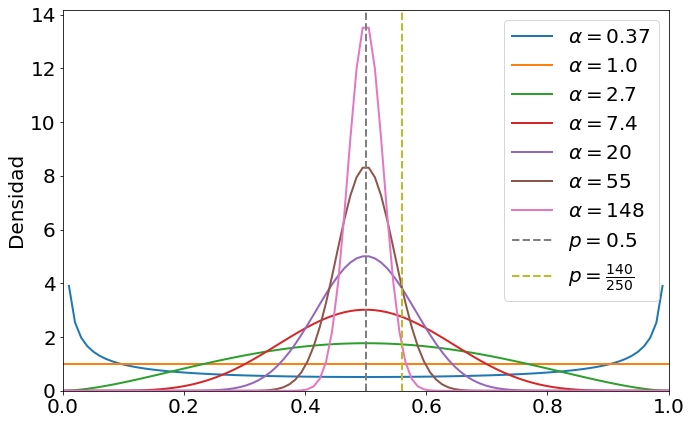
\includegraphics[width=0.55\textwidth]{betas}} \\
            $1.00$ & $0.48$ \\
            $2.70$ & $0.82$ \\
            $7.40$ & $1.3$ \\
            $20.00$ & $1.8$ \\
            $55.00$ & $1.9$ \\
            $148.00$ & $1.7$ \\
            $403.00$ & $1.3$ \\
            $1096.00$ & $1.1$
        \end{tabular}
    \end{center}
\end{frame}

\begin{frame}
    \frametitle{Enfoque bayesiano}
    \begin{block}{Hipótesis}
        \begin{itemize}
            \item $H_{0}: p = 0.5$, $H_{1}: p \sim \betadist{\alpha}{\alpha}$, $H_{2}: p = \frac{140}{250}$.
        \end{itemize}
    \end{block}
    \begin{center}
        \begin{tabular}{r|lc}
            $\alpha$ & $\frac{\prob{140 \mid H_{1}}}{\prob{140 \mid H_{0}}}$ & Prior (distribución beta $\betadist{\alpha}{\alpha}$) \\
            \hline
            $0.37$ & $0.25$ & \multirow{9}{*}{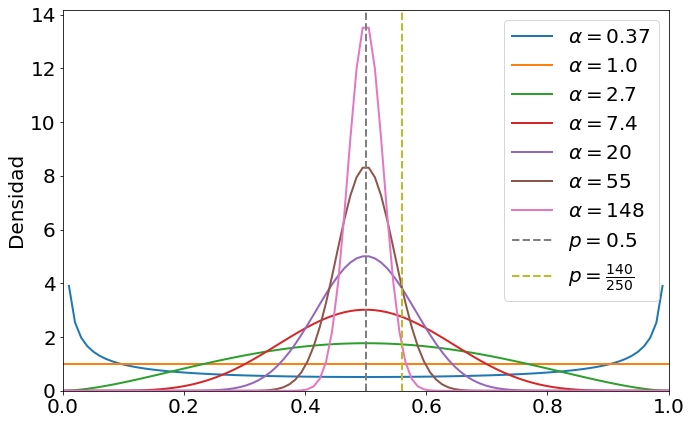
\includegraphics[width=0.55\textwidth]{betas}} \\
            $1.00$ & $\mathbf{0.48}$ \\
            $2.70$ & $0.82$ \\
            $7.40$ & $1.3$ \\
            $20.00$ & $1.8$ \\
            $55.00$ & $\mathbf{1.9}$ \\
            $148.00$ & $1.7$ \\
            $403.00$ & $1.3$ \\
            $1096.00$ & $1.1$
        \end{tabular}
    \end{center}
    \begin{block}{}%Hipótesis}
        \begin{itemize}
            \item $\frac{\prob{140 \mid H_{2}}}{\prob{140 \mid H_{0}}} = \frac{\parens{\frac{140}{250}}^{140} \parens{1 - \frac{140}{250}}^{110}}{\frac{1}{2^{250}}}
                = \frac{2^{250} 140^{140} 110^{110}}{250^{250}} \approx 6.1$.
        \end{itemize}
    \end{block}
\end{frame}

\begin{frame}
    \frametitle{Pequeño cambio}
    \begin{block}{Ejercicio}
        \begin{itemize}
            \item Supongamos moneda sigue una distribución $X \sim \bernoulli{p}$.
            \item $H_{0}: p = 0.5$.
            \item $H_{1}: p \neq 0.5$.
            \item Muestra de tamaño $n = 250$, y se obtienen $141$ caras.
        \end{itemize}
    \end{block}
    \begin{block}{p-valor}
        \begin{itemize}
            \item Según teorema del límite central, $\bar{X}_{n} \sim \normal{\mu}{\frac{\sigma^{2}}{n}}$.
            \item En este caso $\mu = p$, $\sigma^{2} = p \parens{1 - p}$.
            \item Es decir, $\bar{X}_{n} \sim \normal{p}{p \parens{1 - p}}$.
            \item Se calcula $z = \frac{\sqrt{n} \parens{\bar{x}_{n} - \mu}}{\sqrt{\sigma^{2}}} = \frac{\sqrt{n} \parens{\bar{x}_{n} - p}}{\sqrt{p \parens{1 - p}}} = \frac{\sqrt{250} \parens{\frac{141}{250} - 0.5}}{0.5} \approx 2.0239$.
            \item p-valor sería $\prob{\vparens{Z} > z \mid p = 0.5} \approx 0.0430$.
        \end{itemize}
    \end{block}
\end{frame}

\begin{frame}
    \frametitle{Pequeño cambio}
    \begin{block}{Ejercicio}
        \begin{itemize}
            \item Supongamos moneda sigue una distribución $X \sim \bernoulli{p}$.
            \item $H_{0}: p = 0.5$.
            \item $H_{1}: p \neq 0.5$.
            \item Muestra de tamaño $n = 250$.
        \end{itemize}
    \end{block}
    \begin{block}{p-valor}
        \begin{itemize}
            \item Si hay $140$ caras, p-valor es $0.0578$.
            \item Si hay $141$ caras, p-valor es $0.0430$.
            \item Se fija nivel de significancia $0.05$.
            \item En el primer caso, no se rechaza la hipótesis, en el segundo sí.
        \end{itemize}
    \end{block}
\end{frame}

\begin{frame}
    \frametitle{Enfoque bayesiano}
    \begin{block}{Hipótesis}
        \begin{itemize}
            \item $H_{0}: p = 0.5$, $H_{1}: p \sim \betadist{\alpha}{\alpha}$, $H_{2}: p = \frac{140}{250}$, $H_{3}: p = \frac{141}{250}$.
        \end{itemize}
    \end{block}
    \begin{center}
        \begin{tabular}{r|llc}
            $\alpha$ & $\frac{\prob{140 \mid H_{1}}}{\prob{140 \mid H_{0}}}$ & $\frac{\prob{141 \mid H_{1}}}{\prob{141 \mid H_{0}}}$ & Prior (distribución beta $\betadist{\alpha}{\alpha}$) \\
            \hline
            $0.37$ & $0.25$ & $0.32$ & \multirow{9}{*}{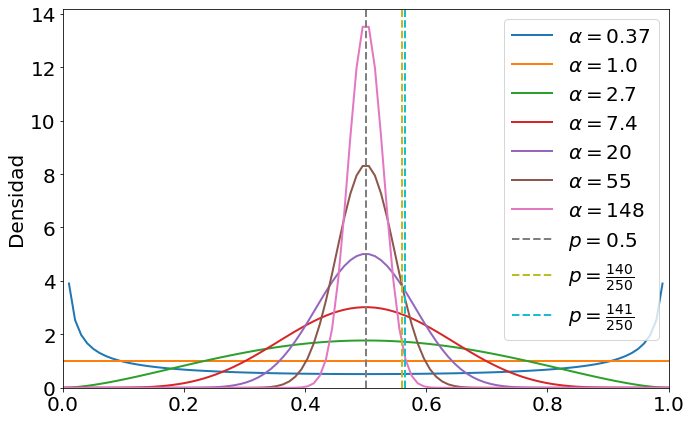
\includegraphics[width=0.52\textwidth]{betas2}} \\
            $1.00$ & $\mathbf{0.48}$ & $\mathbf{0.61}$ & \\
            $2.70$ & $0.82$ & $1.0$ & \\
            $7.40$ & $1.3$ & $1.6$ & \\
            $20.00$ & $1.8$ & $2.2$ & \\
            $55.00$ & $\mathbf{1.9}$ & $\mathbf{2.3}$ & \\
            $148.00$ & $1.7$ & $1.9$ & \\
            $403.00$ & $1.3$ & $1.4$ & \\
            $1096.00$ & $1.1$ & $1.2$ &
        \end{tabular}
    \end{center}
    \begin{block}{}%Hipótesis}
        \begin{itemize}
            \item $\frac{\prob{140 \mid H_{2}}}{\prob{140 \mid H_{0}}} = \frac{2^{250} 140^{140} 110^{110}}{250^{250}} \approx 6.1$,
                y
                $\frac{\prob{141 \mid H_{3}}}{\prob{141 \mid H_{0}}} = \frac{2^{250} 141^{141} 109^{109}}{250^{250}} \approx 7.8$.
        \end{itemize}
    \end{block}
\end{frame}

\begin{frame}
    \frametitle{Enfoque bayesiano}
    \begin{alertblock}{Cuidado}
        \begin{itemize}
            \item A veces se interpreta un p-valor de $0.05$ como que la probabilidad en contra la hipótesis nula es $20$ contra $1$.
            \item En realidad, la evidencia en este caso está ligeramente a favor de la hipótesis nula, o contra de ella a lo más $2.3$ contra $1$, dependiendo del prior.
        \end{itemize}
    \end{alertblock}
    \begin{alertblock}{Cuidado}
        \begin{itemize}
            \item Los p-valores y niveles de significancia hay que tratarlos con \emph{extremo} cuidado.
            \item Muchos grandes enredos en la ciencia han sido producto de malas interpretaciones de p-valores.
            \item Es mucho más común de lo que parece.
        \end{itemize}
    \end{alertblock}
\end{frame}

\begin{frame}
    \frametitle{¿Basta con p-valores?}
    \begin{exampleblock}{Ejemplo}
        \begin{itemize}
            \item Un científico lanza una moneda $12$ veces y obtiene la secuencia $cccsccccsccs$.
            \item La secuencia contiene $3$ $s$ y $9$ $c$.
            \item ¿Es la moneda sesgada?
        \end{itemize}
    \end{exampleblock}
    \begin{block}{p-valor}
        \begin{itemize}
            \item Sea $n = 12$ y $r$ la cantidad de $s$.
            \item $r$ sigue una distribución binomial $\binomial{12}{p}$.
            \item Sea $H_{0}: p = 0.5$.
            \item $\prob{r \leq 3 \mid p = 0.5} = \frac{1}{2^{12}} \sparens{\combin{12}{0} + \combin{12}{1} + \combin{12}{2} + \combin{12}{3}} \approx 0.073$.
            \item Bilateral: $\prob{r \leq 3 \text{ o } r \geq 9 \mid p = 0.5} \approx 0.146$.
        \end{itemize}
    \end{block}
\end{frame}

\begin{frame}
    \frametitle{¿Basta con p-valores?}
    \begin{exampleblock}{Ejemplo}
        \begin{itemize}
            \item El científico dice que la variable aleatoria no es $r$, pues antes de lanzar la moneda, ya había decidido que lo haría hasta que apareciesen $3$ $s$. La variable aleatoria debe ser $n$.
            \item La secuencia contiene $3$ $s$ y $9$ $c$.
            \item ¿Es la moneda sesgada?
        \end{itemize}
    \end{exampleblock}
    \begin{block}{p-valor -- caso 2}
        \begin{itemize}
            \item Sea $r = 3$ y $n$ la cantidad de lanzamientos hasta observar $3$ $s$.
            \item $n$ sigue una distribución con masa $\prob{n \mid p = 0.5 , r} = \combin{n - 1}{r - 1} \parens{\frac{1}{2}}^{n}$.
                \begin{multline*}
                    \prob{n \geq 12 \mid p = 0.5} = \sum_{n = 12}^{+ \infty} \frac{1}{2^{n}} \combin{n - 1}{2}
                    = \sum_{n = 12}^{+ \infty} \frac{\parens{n - 1} \parens{n - 2}}{2^{n + 1}}
                    \\
                    \approx 0.03 .
                \end{multline*}
        \end{itemize}
    \end{block}
\end{frame}

\begin{frame}
    \frametitle{¿Basta con p-valores?}
    \begin{exampleblock}{Ejemplo}
        \begin{itemize}
            \item La secuencia contiene $3$ $s$ y $9$ $c$.
            \item ¿Es la moneda sesgada?
        \end{itemize}
    \end{exampleblock}
    \begin{block}{Enfoque bayesiano -- caso 1}
        \begin{itemize}
            \item Supongamos prior para $p$ como $\betadist{\alpha}{\alpha}$.
            \item Verosimilitud binomial $r \sim \binomial{12}{p}$.
                \begin{multline*}
                    \pdf{p \mid r = 3} = \frac{\prob{r = 3 \mid p} \pdf{p}}{\prob{r = 3}}
                    \\
                    = \frac{\combin{12}{3} p^{3} \parens{1 - p}^{9} \gammafunc{2 \alpha} p^{\alpha - 1} \parens{1 - p}^{\alpha - 1}}{\gammafunc{\alpha}^{2} \prob{r = 3}}
                    \\
                    \propto \frac{\gammafunc{2 \alpha} p^{2 + \alpha} \parens{1 - p}^{8 + \alpha}}{\gammafunc{\alpha}^{2}} .
                \end{multline*}
        \end{itemize}
    \end{block}
\end{frame}

\begin{frame}
    \frametitle{¿Basta con p-valores?}
    \begin{exampleblock}{Ejemplo}
        \begin{itemize}
            \item La secuencia contiene $3$ $s$ y $9$ $c$.
            \item ¿Es la moneda sesgada?
        \end{itemize}
    \end{exampleblock}
    \begin{block}{Enfoque bayesiano -- caso 2}
        \begin{itemize}
            \item Supongamos prior para $p$ como $\betadist{\alpha}{\alpha}$.
            \item Verosimilitud para $n \sim \combin{n - 1}{r - 1} p^{r} \parens{1 - p}^{n - r} = \frac{\parens{n - 1} \parens{n - 2} p^{3} \parens{1 - p}^{9}}{2}$.
                \begin{multline*}
                    \pdf{p \mid n = 12} = \frac{\prob{n = 12 \mid p} \pdf{p}}{\prob{n = 12}}
                    \\
                    = \frac{\parens{12 - 1} \parens{12 - 2} p^{3} \parens{1 - p}^{9} \gammafunc{2 \alpha} p^{\alpha - 1} \parens{1 - p}^{\alpha - 1}}{2 \gammafunc{\alpha}^{2} \prob{n = 12}}
                    \\
                    \propto \frac{\gammafunc{2 \alpha} p^{2 + \alpha} \parens{1 - p}^{8 + \alpha}}{\gammafunc{\alpha}^{2}} .
                \end{multline*}
        \end{itemize}
    \end{block}
\end{frame}

\begin{frame}
    \frametitle{¿Basta con p-valores?}
    \begin{alertblock}{Enfoque bayesiano}
        \begin{itemize}
            \item ¡No depende de la decisión de cómo se tomó la muestra!
        \end{itemize}
    \end{alertblock}
    \begin{block}{Para convencerse}
        \begin{itemize}
            \item Un espía revisa resultados obtenidos para cada lanzamiento en la medida que ocurren.
            \item ¿La inferencia del espía en cada lanzamiento debería depender del criterio de término del experimento?
        \end{itemize}
    \end{block}
    \begin{block}{Para convencerse 2}
        \begin{itemize}
            \item Luego del lanzamiento $12$, alguien entra al laboratorio y roba la moneda.
            \item Ya no se pueden realizar más experimentos, por lo que aunque se haya querido, no se pueden hacer más lanzamientos.
            \item ¿Cómo se calcula el p-valor en ese caso?
        \end{itemize}
    \end{block}
\end{frame}

\iffalse
\begin{frame}[allowframebreaks, noframenumbering]
\frametitle<presentation>{References}
\printbibliography
%\bibliographystyle{apalike}
\end{frame}
\fi

\end{document}
